\section{Construct Environment 3D Models}\label{sec:construct-environment}
\subsection{Problem Statement}
For the AR application to track the environment, a 3D model of the indoor environment must be predefined and imported as an Area Target. We need a method for constructing a fast, easy, cost-efficient model that can be executed on mobile devices.

\subsection{Solution: Vuforia Creator Application}
Vuforia provides the Vuforia Creator application, which is available on the App Store for iOS devices. With the application installed on an iPad or iPhone, a medium-sized indoor environment of about $50m^2$—for example, one level of the I building at HCMUS—can be scanned manually, and the entire process can be completed in 20 minutes.

\subsubsection{Scan an Environment}
Before scanning, a path around the area should be planned, which will be followed during the scanning session. Once a new location is selected for capture in the Vuforia Creator application, the mobile device's camera will be activated and ready to scan, as shown in Figure~\ref{fig:construct-environment-1}. A live green mesh overlay indicates which parts have been scanned and whether the scanning angles and shapes are sufficiently accurate.

\begin{figure}[ht]
  \centering
  \includegraphics[scale=0.1]{content/resources/images/chap-problems-solutions/construct-environment-1.PNG}
  \caption{Scanning an environment with Vuforia Creator App.}
  \label{fig:construct-environment-1}
\end{figure}

It is advisable to move the mobile camera slowly through the area during the scanning session, scanning the path most carefully to ensure that the resulting model is constructed accurately and smoothly for navigation. Individual objects in the environment, especially the distinctive ones, should also be scanned meticulously to support the tracking quality between similar scenes. This casual scanning of objects provides sufficient information for the AR application to detect and register the area.

If the camera is moved too suddenly, the application might lose track of the environment. In such cases, the system prompts the user to return to an already scanned region to re-establish tracking, as shown in Figure~\ref{fig:construct-environment-2}.

\begin{figure}[ht]
  \centering
  \includegraphics[scale=0.1]{content/resources/images/chap-problems-solutions/construct-environment-2.PNG}
  \caption{Vuforia Creator App prompts the user to return to a scanned area.}
  \label{fig:construct-environment-2}
\end{figure}

The scanning session takes about 15 minutes.

\subsubsection{Construct Scanned Model and Import}
Once the scanning session is finished, the user can export the captured data in one of two formats: as a raw 3D model or as an Area Target. Exporting as an Area Target is especially beneficial, as it generates a Unity package that can be directly imported into Unity projects, simplifying the integration process. The entire generation process typically takes up to 5 minutes to complete, depending on the complexity of the scanned environment.

Once the Area Target is successfully generated and imported, it will appear as an object within the Unity project. The imported Area Target will be displayed at the correct scale, accurately reflecting the proportions of the real-world environment without additional adjustments, as shown in Figure~\ref{fig:construct-environment-4}.

\begin{figure}[ht]
  \centering
  \includegraphics[scale=0.1]{content/resources/images/chap-problems-solutions/construct-environment-3.PNG}
  \caption{Generating model.}
  \label{fig:construct-environment-3}
\end{figure}

\begin{figure}[ht]
  \centering
  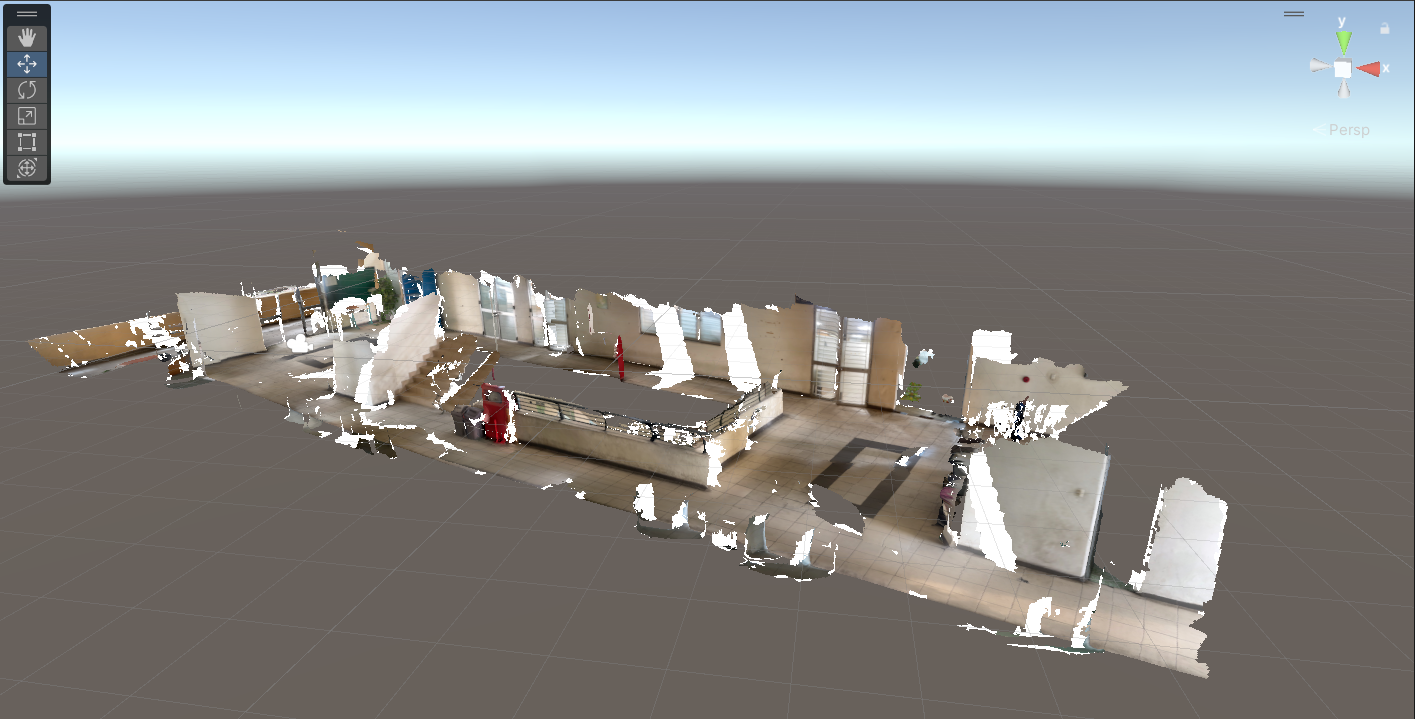
\includegraphics[scale=0.3]{content/resources/images/chap-problems-solutions/construct-environment-4.PNG}
  \caption{A scan of the 8th floor of building I at HCMUS.}
  \label{fig:construct-environment-4}
\end{figure}

\subsubsection{Multiple Areas}
Since the scanning area is limited, we need to create multiple models and merge them for a larger space—specifically, the I building. Fortunately, the Vuforia Creator application supports capturing adjacent areas. Once we have the 3D model of an area, we can continue scanning the neighboring area by selecting \textit{Capture Aligned Area}. After that, we must re-scan approximately $25\%$ of the current area that overlaps with the adjacent area so that the application can automatically scale it. This process can be repeated until the entire spacious area is fully scanned. All the separate scanned models will be automatically scaled and correctly aligned with each other once imported into the Unity project as Area Targets. Figure~\ref{fig:construct-environment-5} shows the 7th and 8th floors of the I building at HCMUS, constructed by three separate scans.

\begin{figure}[ht]
  \centering
  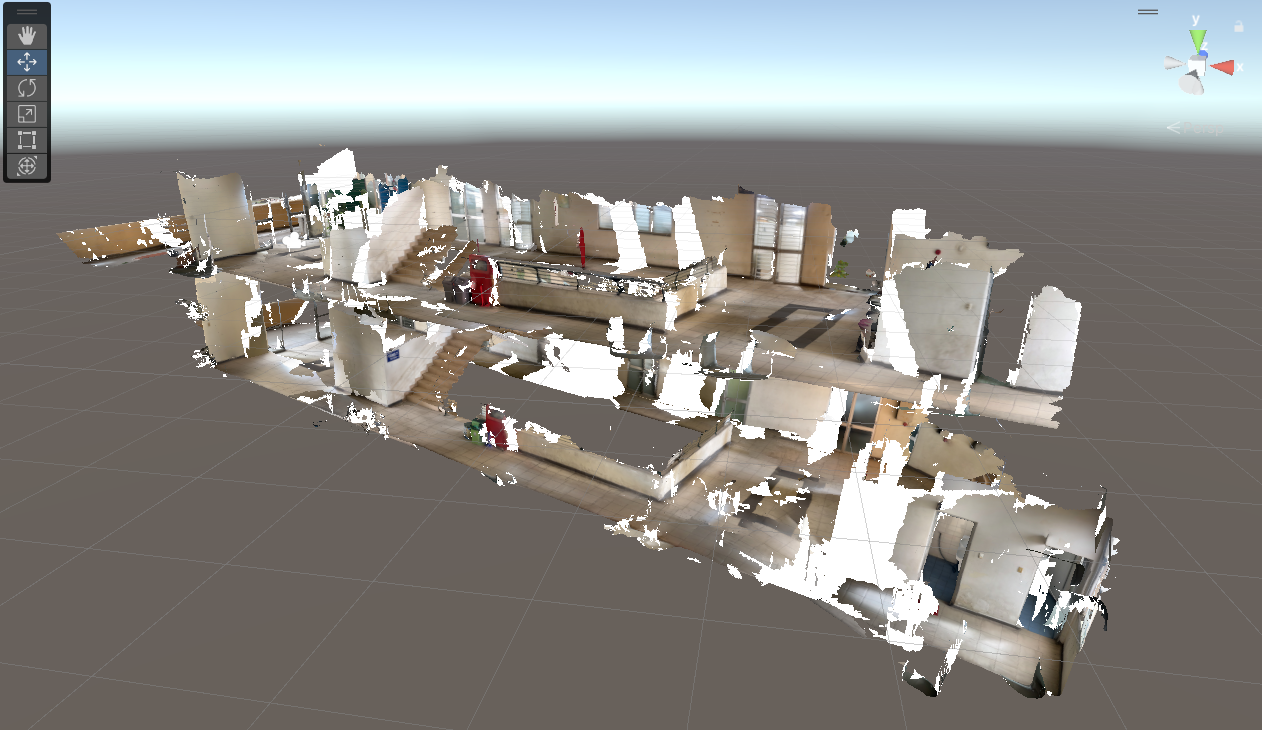
\includegraphics[scale=0.3]{content/resources/images/chap-problems-solutions/construct-environment-5.PNG}
  \caption{Combination of scans from the 7th and 8th floors of building I at HCMUS.}
  \label{fig:construct-environment-5}
\end{figure}

\begin{figure}[ht]
  \centering
  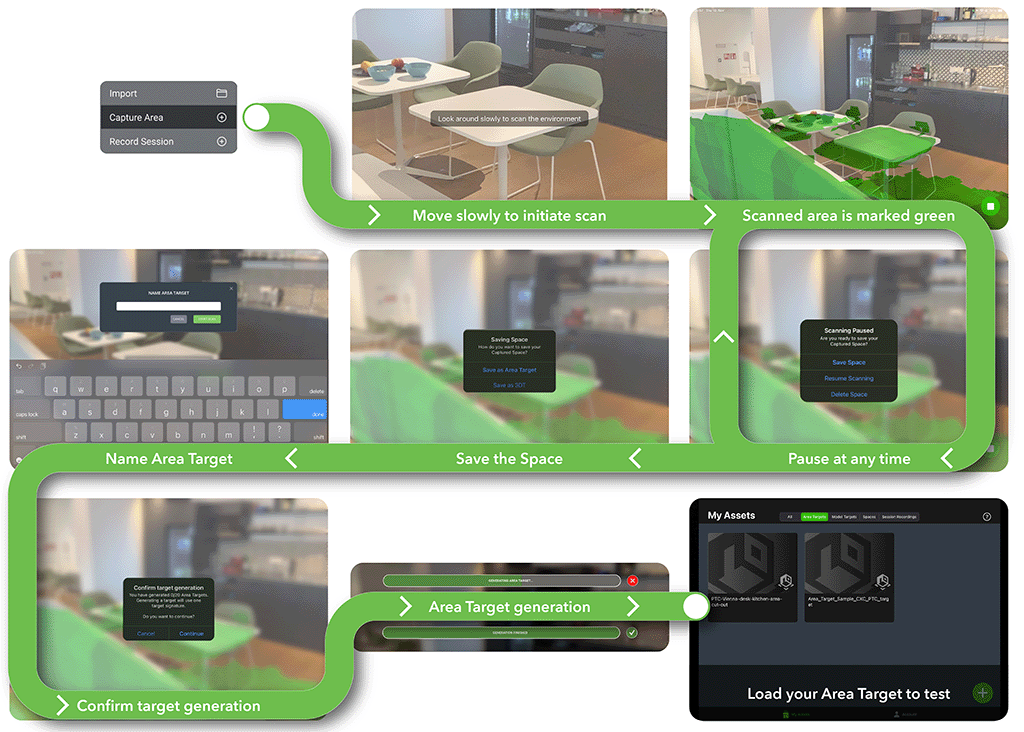
\includegraphics[scale=1]{content/resources/images/chap-problems-solutions/construct-environment-6.PNG}
  \caption{The workflow of generating a scan. \\ \small{Source: \url{https://developer.vuforia.com/library/tools/creator-app}}}
  \label{fig:construct-environment-6}
\end{figure}
